\documentclass[10pt,letterpaper]{article}

\usepackage[utf8]{inputenc}
\usepackage[spanish,es-nodecimaldot]{babel}
\usepackage{amsmath}
\usepackage{amssymb}
\usepackage{graphicx}
\usepackage{mathtools}

\usepackage{multicol}

\usepackage{enumitem}

\usepackage[top=1in, bottom=1in, left=1in, right=1in]{geometry}

\renewcommand{\arraystretch}{1.5}

\begin{document}

\begin{titlepage}
    \centering

    {\scshape\LARGE Universidad Nacional Autónoma de México \par}

    \vspace{1cm}
    {\scshape\Large Facultad de Ciencias\par}
    \vspace{1.5cm}

    \begin{center}
        
\includegraphics[scale=.1]{../../assets/img/logo.png}
    \end{center}

    \vspace{.8 cm}

    {\LARGE Tarea 06: \par}
    {\huge\bfseries Estrategias evolutivas\par}

    \vspace{0.5cm}
    \large{\itshape{Pablo A. Trinidad Paz}} \small{ - 419004279}

    \vfill

    Trabajo presentado como parte del curso de
    \textbf{Cómputo Evolutivo}
    impartido por el profesor \textbf{Mario Iván Jaen Márquez}. \par
    \vspace{0.5cm}
    Fecha de entrega: \textbf{Jueves 4 de Abril de 2019}.
\end{titlepage}

\begin{enumerate}
    \item \textbf{[Ejercicio de programación]} Escribe una función que genere números
          pseudo-aleatorios de las distribución normal estándar $N(0, 1)$ a partir de
          números uniformemente distribuidos. Indica el método usado. \\[\baselineskip]

        \textbf{Solución:} Se implementó el método de muestreo de números pseudo-aleatorios
        descrito por Box-Muller\footnote{https://en.wikipedia.org/wiki/Box-Muller\_transform}.
        A continuación se presentan los resultados de la implementación comparados con el
        método $\mathrm{random.gauss(0, 1)}$ de la librería estándar de Python.
        \begin{center}
            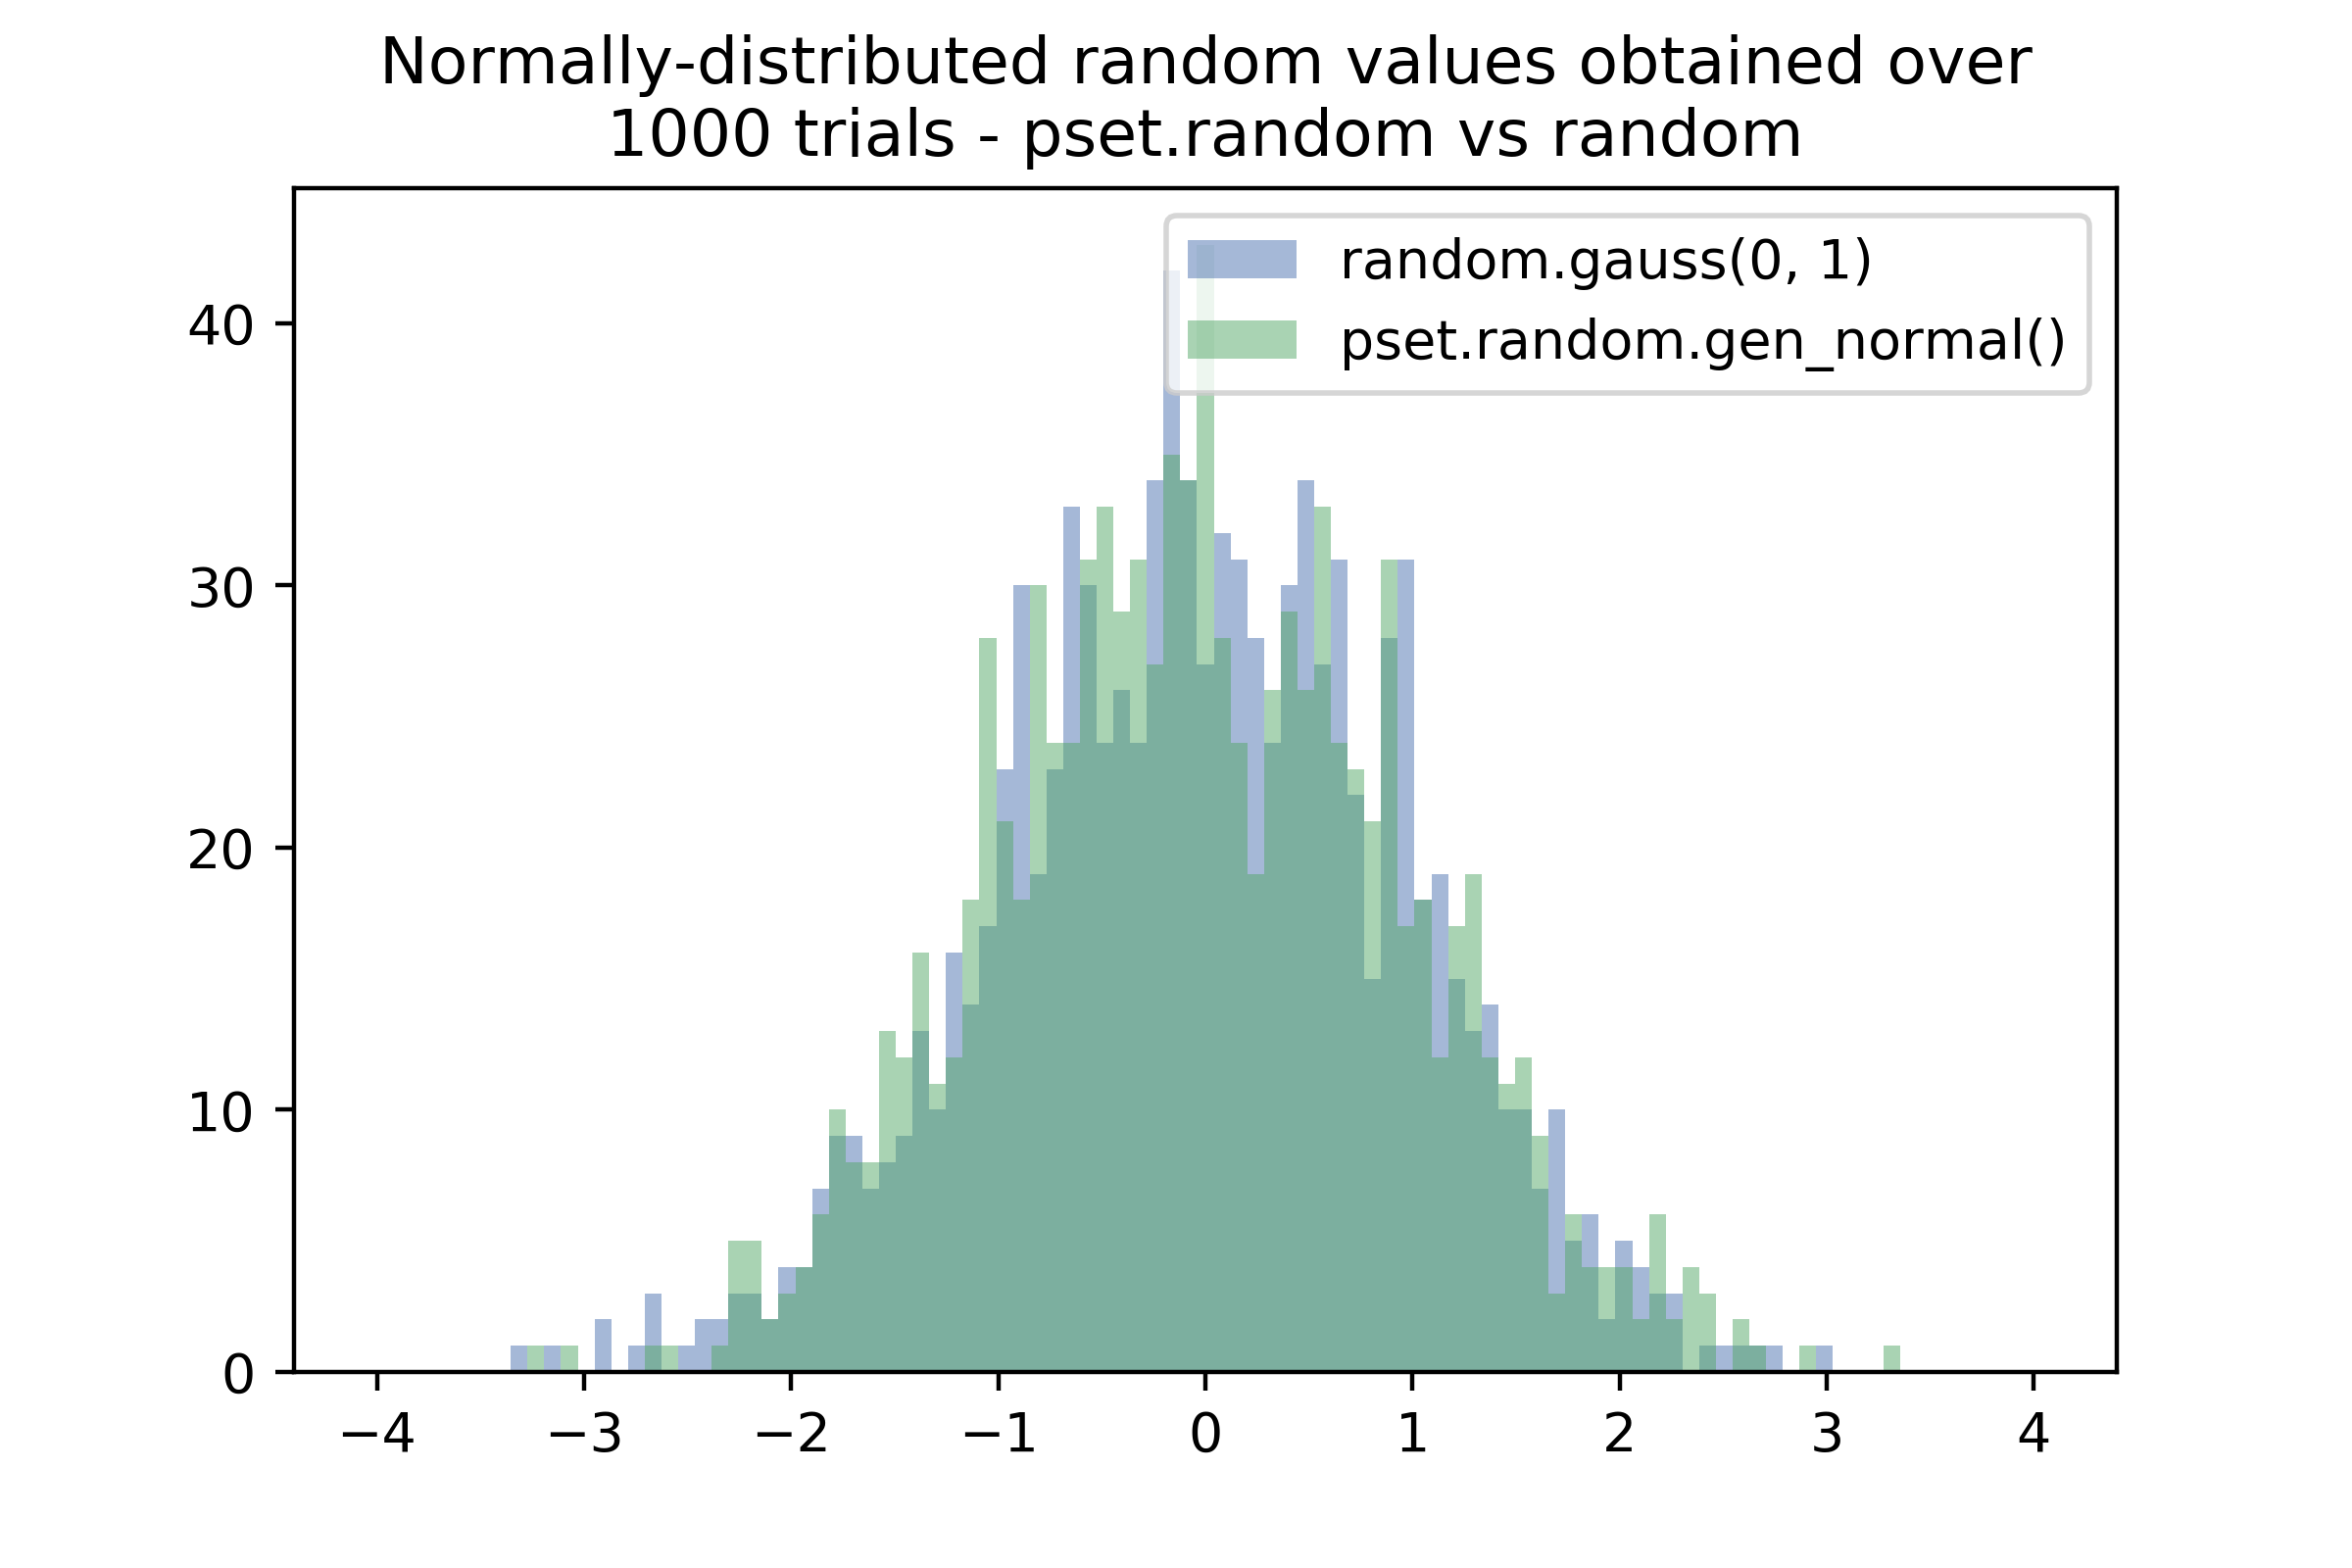
\includegraphics[scale=.6]{./assets/ex1-results1.png}
        \end{center}
        \begin{center}
            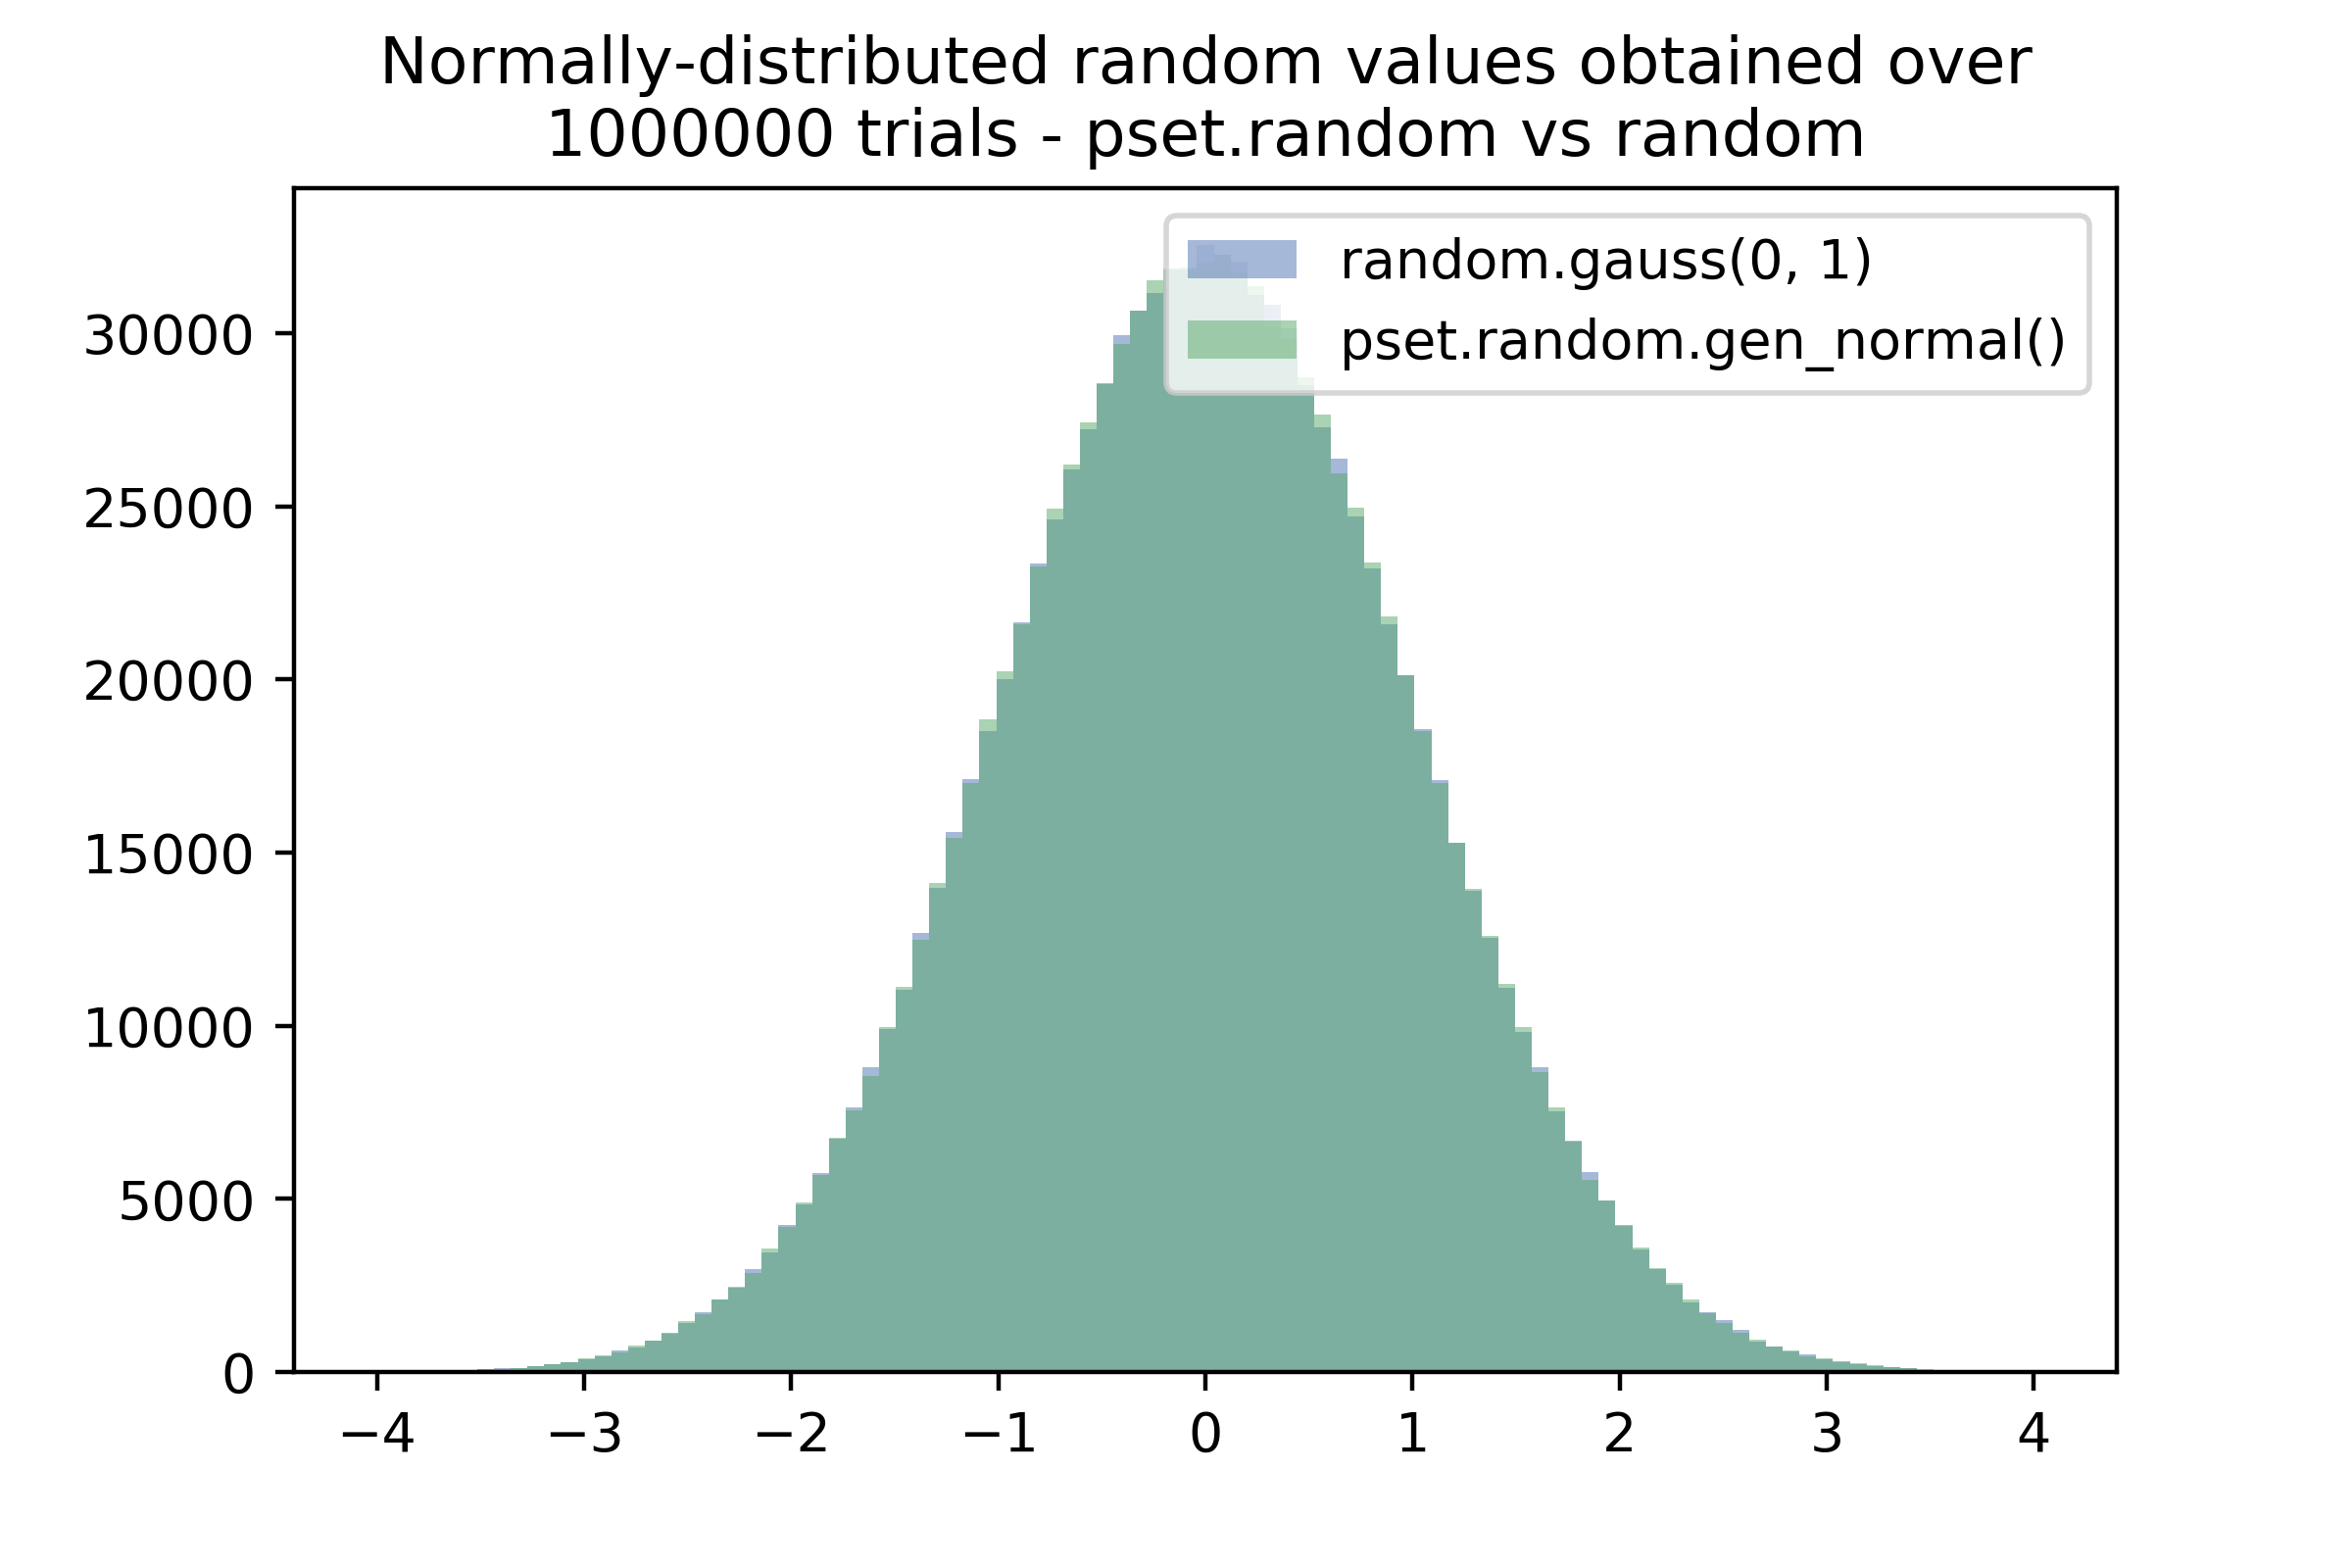
\includegraphics[scale=.6]{./assets/ex1-results2.png}
        \end{center}

    \clearpage
    \item \textbf{[Ejercicio de programación]} Implementa el algoritmo (1+1)-ES. Prueba
          tu algoritmo sobre la función \textit{Sphere}, la cuál es una función unimodal
          $d$-dimensional definida como:

        \begin{equation*} \begin{split} \begin{gathered}
            f(\vec{x}) = \sum_{i=1}^d x_i^2
        \end{gathered} \end{split} \end{equation*}

        Donde cada $x_i \in [-100, 100]$. Utiliza un parámetro $\sigma = 1$ y un punto
        inicial $\vec{x} = (x_1, ..., x_d) = (-99,...,-99)$

        \begin{enumerate}
            \item Ejecuta tu algoritmo para $d=10$ y para $d=100$. ¿Qué tan cerca del óptimo
            converge y qué tan rápido?

            \textbf{Respuesta:} Para $d=10$ con una precisión de $0.01$, el algoritmo converge
            después $391$ mutaciones exitosas con un valor promedio para cada $x_i$ de $0.00263$.
            Para $d=100$ con la misma precisión, el algoritmo converge después de $1337$
            mutaciones con un valor promedio para cada $x_i$ de $0.1486$.

            \item Implementa la regla del $1/5$ y vuelve a ejecutar tu algoritmo. ¿Qué diferencias
            observas respecto a la ejecución anterior?

            \textbf{Respuesta:} La diferencia sólo se notó en el número de mutaciones exitosas
            siendo reducido a $374$ con $d=10$ y un $x_i$ promedio de $-0.1249$ y para $d=100$
            un número de mutaciones exitosas $1211$ con un $x_i$ promedio de $-0.03162$.
        \end{enumerate}

        \begin{center}
            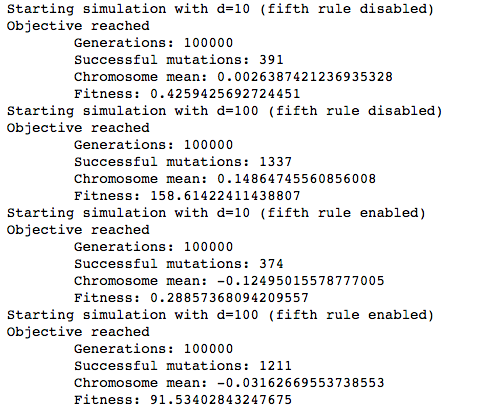
\includegraphics[scale=.6]{./assets/ex-2.png}
        \end{center}
\end{enumerate}

\end{document}